
\documentclass[16pt,twocolumn,letterpaper]{article}
\usepackage{apacite}
\usepackage{tablefootnote}
\usepackage{titling}
\usepackage{graphicx}
\usepackage[T1]{fontenc}
\usepackage{babel}

\usepackage{titlesec}% http://ctan.org/pkg/titlesec
\titleformat{\section}%
  [hang]% <shape>
  {\normalfont\bfseries\Large}% <format>
  {}% <label>
  {0pt}% <sep>
  {}% <before code>
\renewcommand{\thesection}{}% Remove section references...
\renewcommand{\thesubsection}{\arabic{subsection}}%

\setlength{\droptitle}{-12em}  
\setlength\bibitemsep{\baselineskip}
\title{Experimenting with Scaleable Forecasting Models}

\author{
    Matthew Coghlin\\
  	\and
  	Pelumi Dacosta\\
    \and
    Joseph Despres\\
    \and
    Aneesh Gahi\\
    \and
    Joseph Sigler\\
}

\begin{document}

\maketitle
\bibliographystyle{apacite}


\section{Introduction}

Organizations planning for the future need a way of estimating the future value of many things. From estimating retail demand to plan inventory such as inventory, to customer arrivals for staffing decisions, and estimating input costs for budgeting, all depend on forecasts. Forecasting is the practice of using current data available to estimate the value of a future variable at a time that has not yet happened. Decision makers in government, businesses, and non-profit organizations all require accurate and reliable forecasts. However, there are tremendous costs associated with forecasts that are either too high or too low. This could mean a store running out of inventory, unable to checkout enough shoppers, or be left with rotting produce. Therefore, it is essential to minimize forecasting error. However, there is a growing number of items to forecast and manually forecasting each series will not scales. Therefore, this project implements methods for generating high quality, reliable forecasts for many series. 

As data becomes cheaper to store and more convenient to collect, organizations have the opportunity to get better data driven forecasts. To obtain accurate, reliable, and interpret able forecasts in the past, a time-series expert was generally required to carefully tune model parameters \cite{taylor2018forecasting} and make judgments on which models to implement. Although, this approach is rigorous, it does not scale. Any standard grocery store has enough items to overwhelm anyone manually tuning and selecting forecasting models. Analysts could be asked to generate high quality forecasts for thousands, and even hundreds of thousands of series at a time. The goal of this project is to implement forecasting algorithms that generate high quality forecasts with minimal involvement, validate them with a training and testing partisan, and generate ensemble predictions made up of the various forecasts.

We begin with a discussion of the data and metrics used to evaluate forecasts. Then we specify the requirements for the models to be used for this task. Then we briefly explain the intuition of each model and some reasons for selecting them. Then we discuss the models performance on testing data. After that we discuss our Kaggle challenge and the various approaches we took when making submissions. After that, we conclude with some remarks on the process and how these applications could be used in industry.\footnote{Find the code and data used for this project \url{https://github.com/despresj/Data-Mining-Proj}  } 

\section{Data}

The data obtained for this project are provided as part of a Kaggle challenge where participants are to forecast daily retail sales demand \cite{kaggle}. As contestants, we are given 5 years of training data, with the daily sales of 50 different products from ten different stores. This is a total of 913,000 data points to train forecasting models. The goal is to forecast the next 90 days for each of the 50 products and 10 stores. Judged by Symmetric Mean Absolute Percentage Error (SMAPE) shown in Equation 1

\begin{equation}
\textrm{SMAPE}={\frac {100\%}{h}}\sum _{t=1}^{h}{\frac {\left|\hat{y}_t-y_t\right|}{(|y_t|+|\hat{y}_t|)/2}}.
\end{equation}

Where $y_t$ is the actual value, $\hat{y}_t$ is the point forecast, and $h$ is the forecast horizon. This metric is used the account for the different magnitudes of many series to give a fair comparison. Should one use Mean Absolute Percentage Error, there is an asymmetry as forecasting low is penalized more than forecasting high as well as errors in a series with a lower number of units \cite{hyndman2006another}.

The data require very little preparation. There were several data points that were zero which we switched to one because one of the algorithms did not support 0 values. After that we combined the stores and items into one string column to avoid nesting loops when iteration over stores and items. Figure 1 contains a small subset of the series. This subset of the data are highly seasonal with a slight upward trend and Gaussian noise.

After that, we separated data into training and testing partisans to compare model performance. We selected the first 1,279 data points or 80\% training set of our time-series. Then we use the remainder of the data as a testing set. This prepares us to experiment with the models and compare performance. 

\begin{figure}[!htb]
	\center{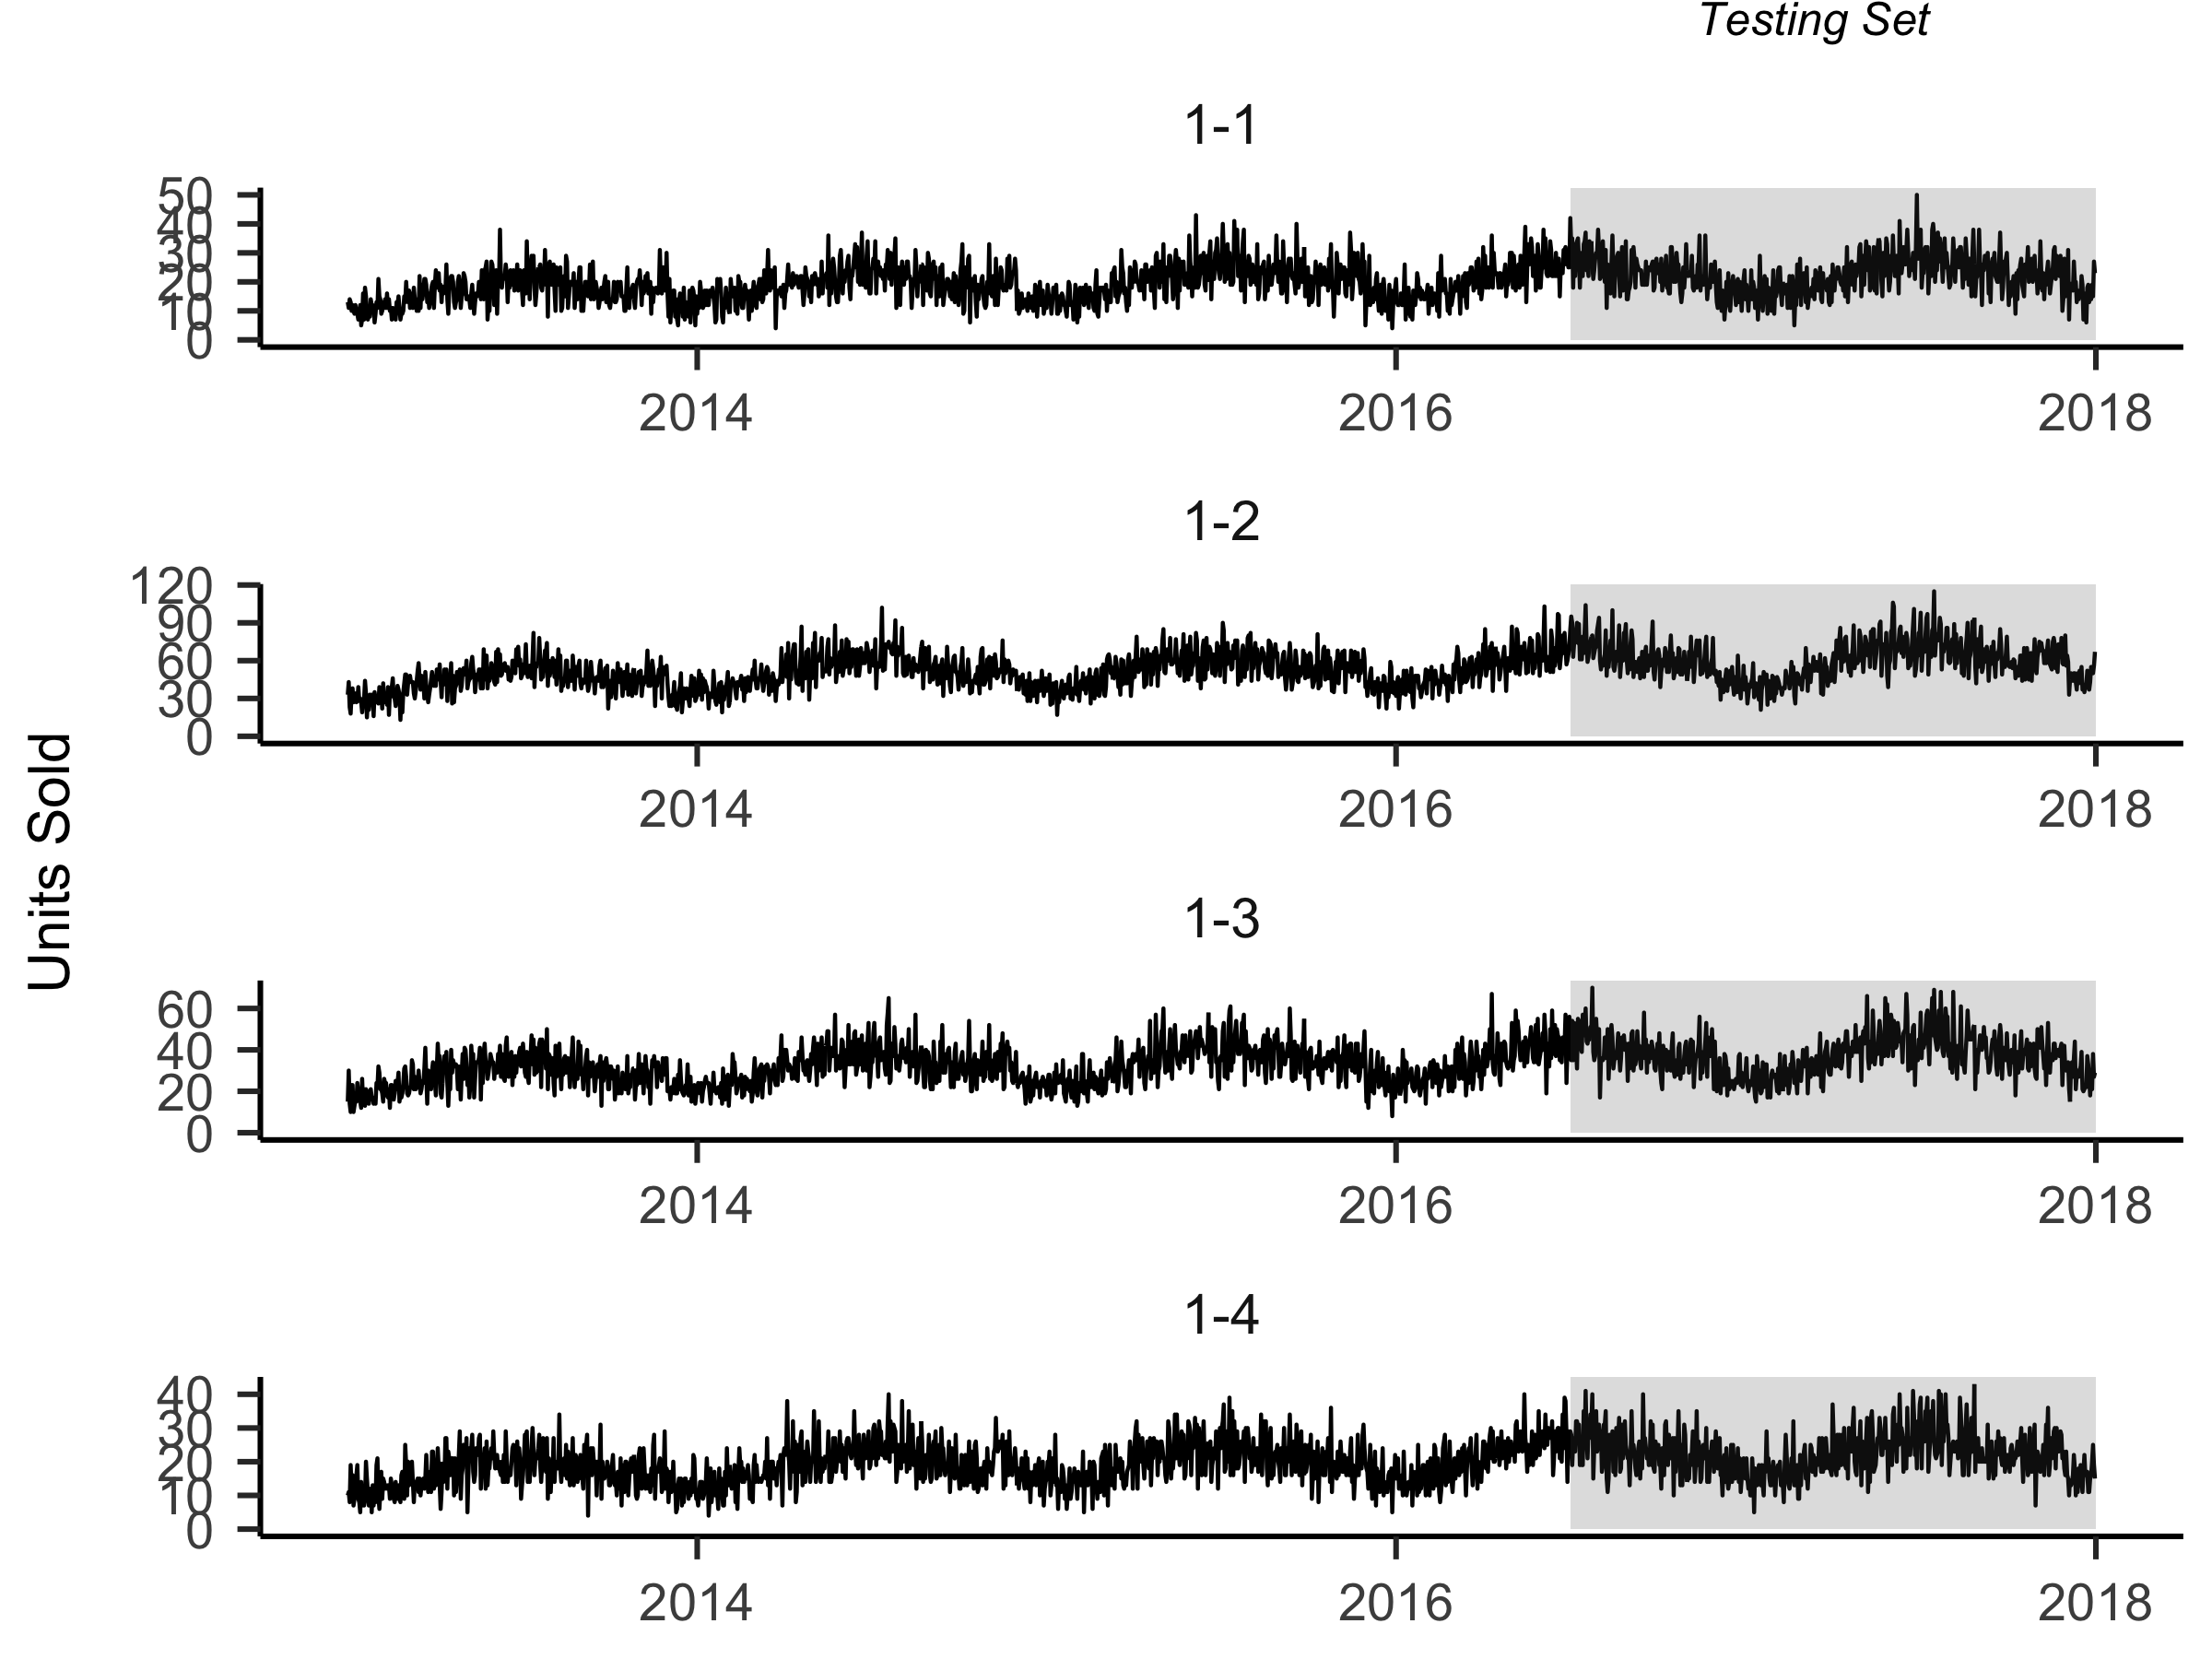
\includegraphics[width=\columnwidth]
        {plots/item_sales.png}}
	\caption{\label{fig:my-label} Daily Sales of the First Four Items in the First store}
\end{figure}

\section{Requirements}

The algorithms we select to generate high quality forecasts will have strictly required to be fast, accurate, and interpretable. To be fast, the models must have minimal hyper parameters to tune or be accurate with some specified default parameters. Grid searching model parameters over many series is not feasible. If these alogrythms are fast, they can be ran on a wide variety of timeseries. That gives analysis and stakeholders a very good idea of what kind of performance to expect. Due to the high costs associated with forecasting errors, these models must be interpretable in the event a steakholder has concerns with the output of a model. 

\section{Models}

There are many forecasting models, however we selected models that have been shown to perform well in practice and fit our project requirements. We choose to test two categories of models. First, classical models that have been successfully implemented with years of good results. They are derrived with statistical methods and have strong theoretical justifications. Second, are newer machine learning based models. This is an open field and we are going to test different models and evaluate them strictly on their performance on testing data. 


\begin{table*}[t] \centering 
  \caption{Forecasting Model Performance} 
  \label{} 
\begin{tabular}{@{\extracolsep{5pt}} lrrr} 
\\[-1.8ex]\hline 
\hline \\[-1.8ex] 
Model & Daily Forecast & Aggregated Weekly & Aggregated Monthly \\ 
\hline \\[-1.8ex] 
FB Prophet & $12.890$ & $7.330$ & $4.240$ \\ 
ARDL & $16.830$ & $8.940$ & $4.480$ \\ 
Neural Prophet & $18.440$ & $10.460$ & $7.610$ \\ 
Exponential Smoothing & $19.310$ & $14.880$ & $13.540$ \\ 
Autoregression & $23.930$ & $17.510$ & $16.250$ \\ 
Xgboost & $30.350$ & $28.850$ & $28.430$ \\ 
\hline \\[-1.8ex] 

\footnotesize{Note: Measured in SMAPE see Equation 1}\\
\end{tabular} 
\end{table*} 

\begin{enumerate}
\item Seasonal Exponential Smoothing
\item Vector Autoregression
\item Autoregressive Distributed Lag
\item XGBoost 
\item Prophet
\item Neural Prophet
\end{enumerate}

\subsection{Seasonal Exponential Smoothing}

The Seasonal Exponential smoothing model, sometimes known as the Holt-Winters method, decomposes the timeseries into three components: Linear Seasonality, Linear Trend, and Gaussian noise \cite{hyndman2018forecasting}. This is a simple, interpretable model, that is fast to impliment and has proven quite reliable.

\subsection{Vector Auto Regression}

The first algorithm we implement, is an autoregressive model. This takes the first 5 lag positions and uses them as regressors, then using timeseries decomposition, it models the seasonality\cite{hamilton1994}. This model is commonly used to forecast economic variables.

\subsection{Auto Regressive Distributed Lag}

ARDL models add to the above auto regressive model, however in addition to seasonality with is fit with a vector of indicator variables. and trend, in this case we are adding an explanatory variable of time and fitting the model to laggs of time.

Although there are many forecasting models to choose from, there is not much research on when a given forecasting model outperforms another. Due to the data having strong weekly swings, we implement several models with an autoregressive terms.


\subsection{XGBoost}

XGBoost is an implementation of a tree boosting system. This uses decsision tree regression, and fits an ensemble of models fit to the data, then the residuals, then fits the residuals residuals. This ensamble of tree boosting is quite robust and is useful for a variety of different regression and classification tasks\cite{chen2015xgboost}.

\subsection{Facebook's Prophet}

Facebook released a forecasting library designed specifically to meet the challenges of generating many high quality forecasts. The model prophet is a General Additive model, that consists of three functions, trend which fits a periodic logistic population growth model (we did not limit the growth, however that is a parameter), seasonality is a Fouire series fit to the remaining seasonal component, and a holiday parameter which is a vector of user specified holiday periods, the holliday periods saw a drop in sales, however not enough to justify us specifying specific dates\cite{taylor2018forecasting}. 

\subsection{NeuralProphet}

NeuralProphet, is a forecasting library that expanding on Facebook's prophet. It does so by including an autoregressive term in the general additive model and uses neural networks to generate the autoregressive terms in the model \cite{triebe2021neuralprophet}.

\section{Performance}
\begin{table*}[ht] 
\centering 
\caption{Descriptive Statistics} 
  \label{} 
\begin{tabular}{@{\extracolsep{5pt}} lrrrr} 
\\[-1.8ex]\hline 
\hline \\[-1.8ex] 
Model & Median & Standard Deviation & 95th Percentile & 5th Percentile \\ 
\hline \\[-1.8ex] 
AR Distributed Lag & $$-$2.861$ & $10.505$ & $12.472$ & $$-$21.776$ \\ 
Exponential Smoothing & $0.704$ & $14.098$ & $26.306$ & $$-$20.514$ \\ 
Neural Prophet & $6.863$ & $10.874$ & $27.095$ & $$-$8.262$ \\ 
Prophet & $0.731$ & $8.660$ & $14.355$ & $$-$13.956$ \\ 
Vector Autoreg & $$-$7.500$ & $14.374$ & $12.627$ & $$-$34.667$ \\ 
XGBoost Forecast & $$-$11.973$ & $12.889$ & $3.153$ & $$-$38.347$ \\ 
\hline \\[-1.8ex] 
\footnotesize{}\\
\end{tabular} 
\end{table*} 


Although the Kaggle challenge we are participaing in is asking for a daily sales forecast, we are going to cover aggregated forecast performance because stakeholders are often far more concerned with weekly or monthly forecasts than daily. The selected forecasting models varied in performance quite dramatically. See Table 1 the the SMAPE of each model. First, we speak to the validity of each model given the performance on these testing data. Although there are 500 series, this is retail sales demand and it exhibits similar patterns. Of the selected models Facebook's prophet outperformed the rest at each level of aggregation. This is not surprising as it is percicely designed for the task of forecasting at scale \cite{taylor2018forecasting}. As the level of aggregation increases, we observe lower errors. 

An advantage of forecasting at this scale is that it shows the level of model performance to expect from each model. See histograms of testing set errors in Figure 2. Notice, XGBoost was consistently forecasting lower than the actual value. Where neural prophet was overforecsating. There may be applications where over or underforecasting may be prefered, however we are looking for the most accurate models would prefer those adjustment to be made heuristically. 

\begin{figure}[!htb]
	\center{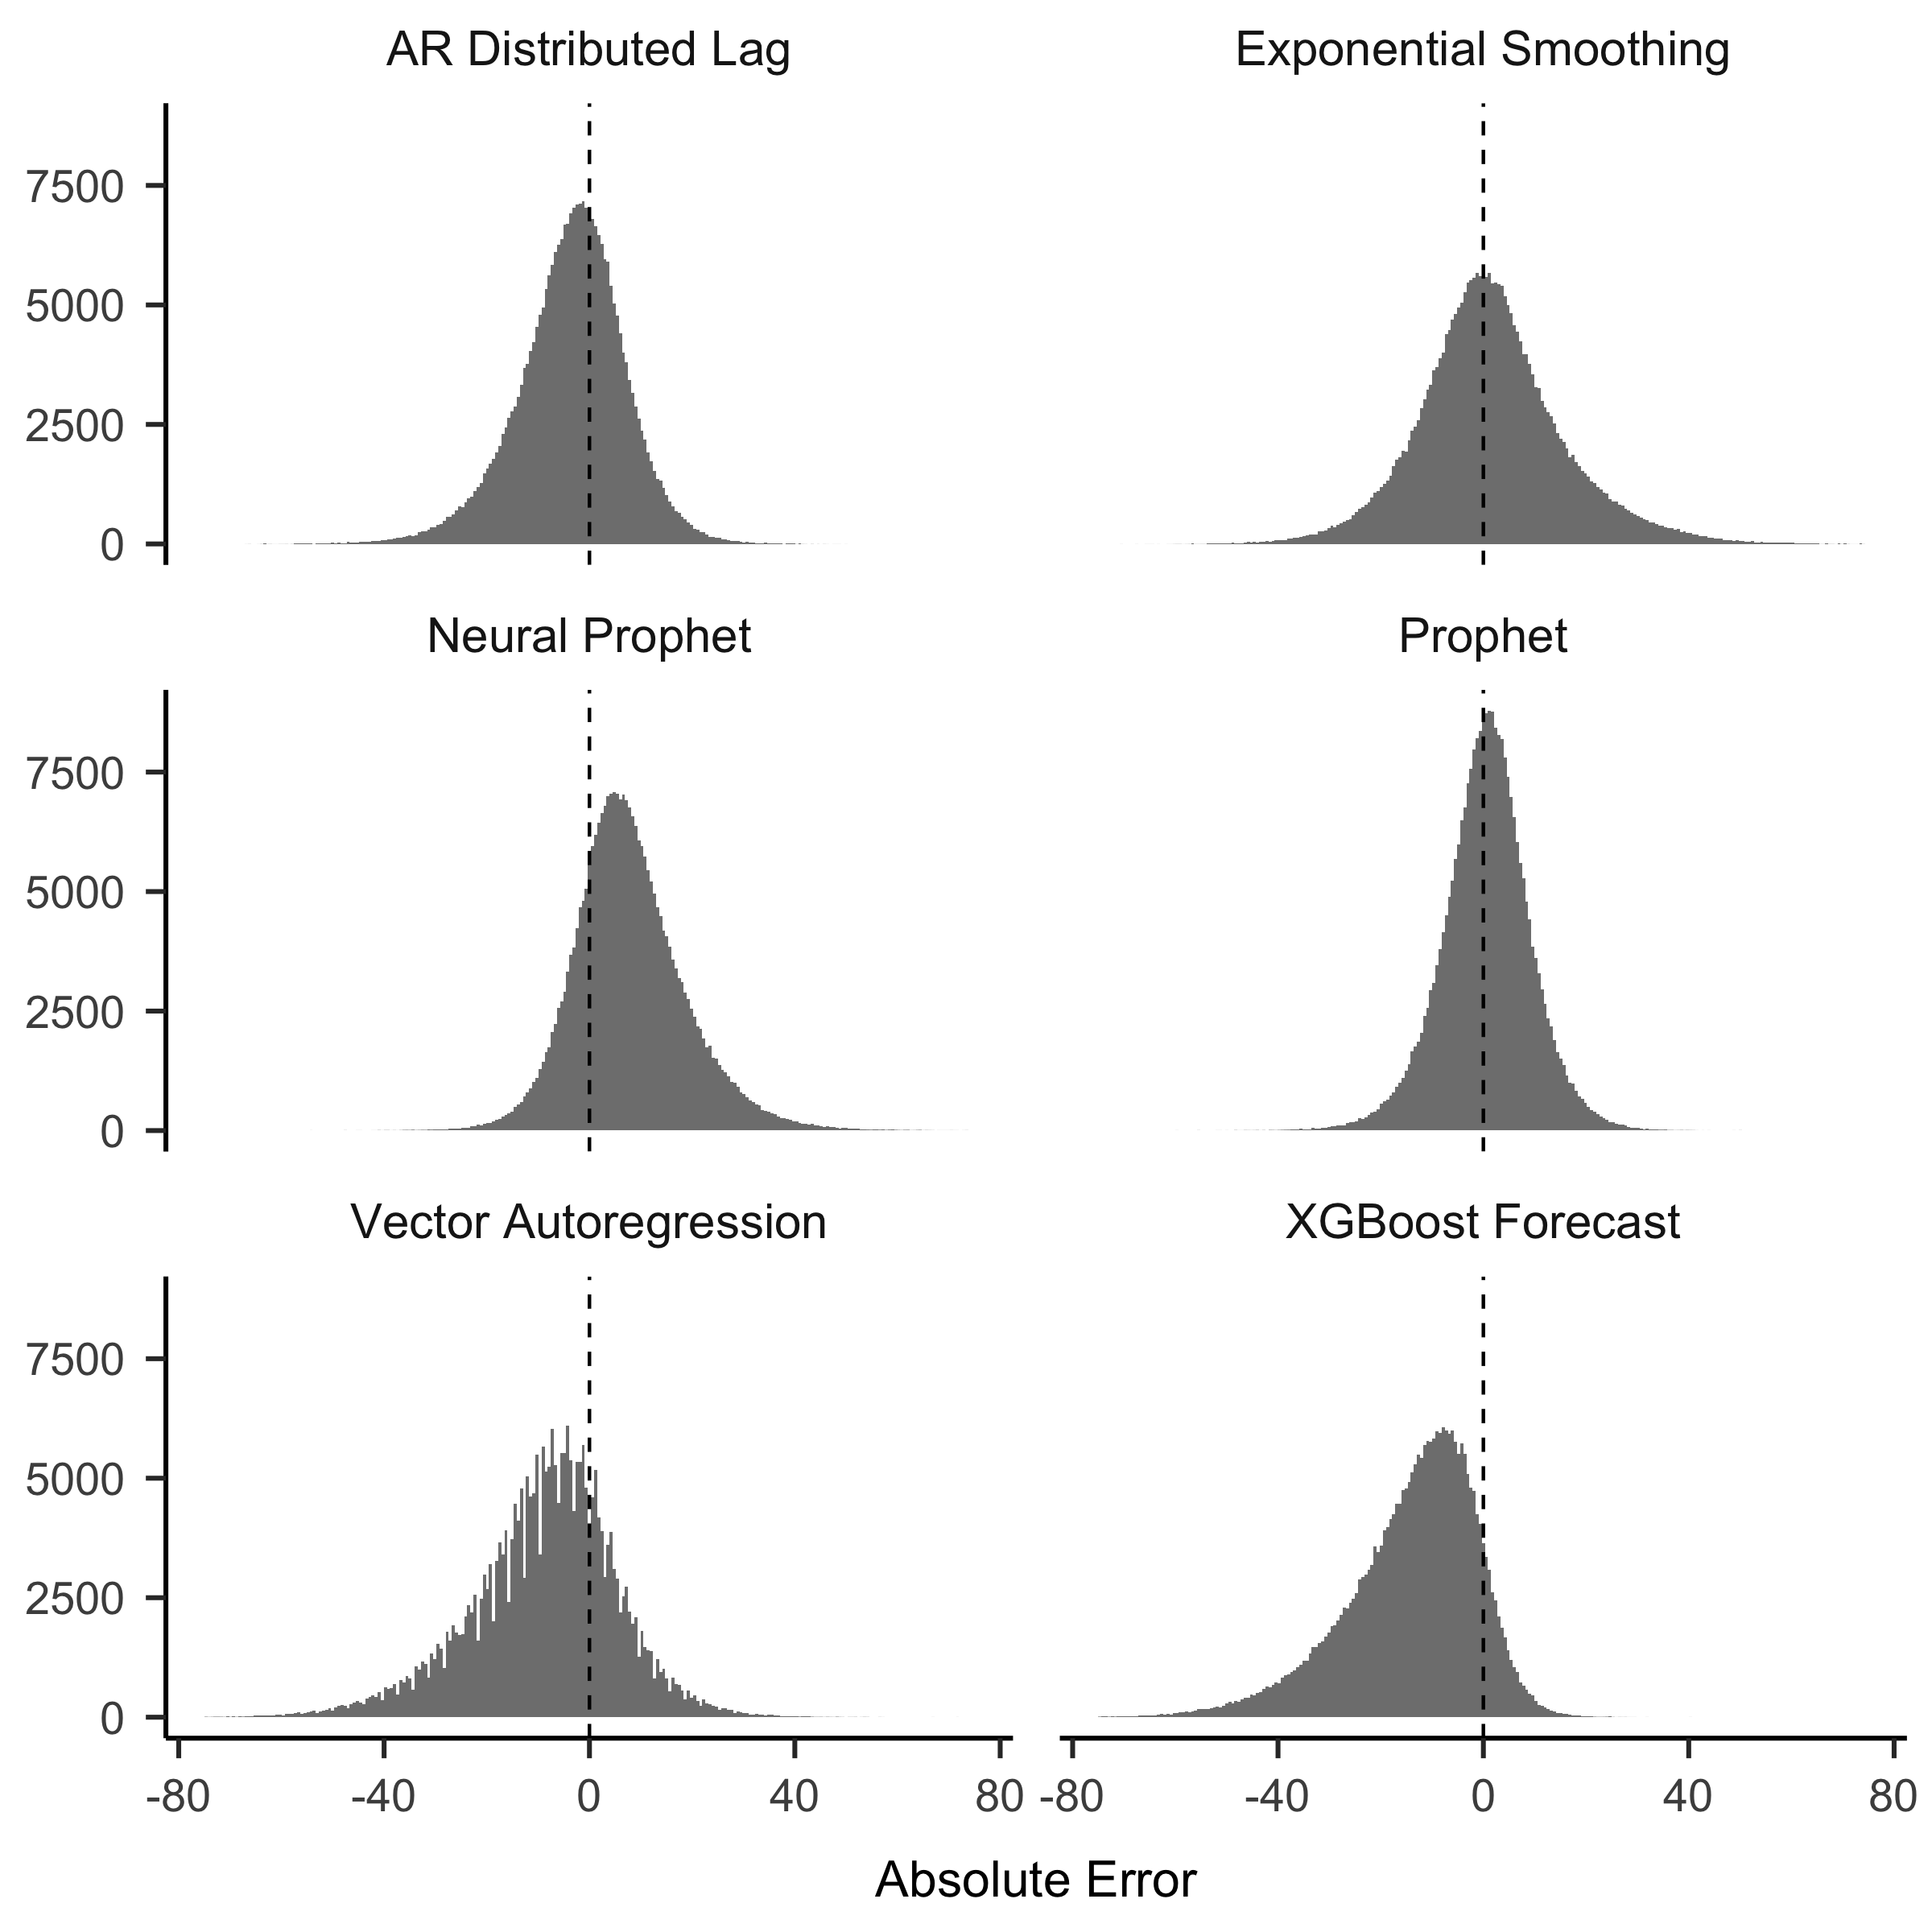
\includegraphics[width=\columnwidth]
        {plots/errors.png}}
	\caption{\label{fig:my-label} Distribution of forecasting errors}
\end{figure}

Table 2 contains descriptive statistics of the each model's performance. Note that the median error of prophet was much lower than in all the other models except for Exponential smoothing. Another consideration is the standard deviation of forecasting errors. This is an important consideration depending on the application. Low standard deviation in forecasting error is highly desirable. The advantage.

Of the models tested, Prophet had the best performance in SMAPE, had the median near zero, and the lowest standard deviation of error. 


\section{Kaggle Challenge}

The challenge is simple generate the best daily forecasts meaured by SMAPE. Since we are not limited in entries we are going to attempt a variety of methods. In this section we will discuss various attempts at this challenge as well as the result. The challenge has passed, so we have access to the leaderboards. The top score is a SMAPE of 12.07 \cite{kaggle}. Therefore, we will compare the models the strategies to that. 

\begin{enumerate}
\item Weight an Average Based on Features
\item Just Use Prophet
\item Ensamble of the Top Three Models
\end{enumerate}

\subsection{Weighted Average}

Improving current models can prove very valueable. Therefore, we will attempt some machine learning methods to combine the models. The goal is to use machine learning to predict when a given forecast. Therefore, we will employ a feature detection algorythm to classify the best model. There are many different shapes and patterns a timerseries plot can take. Seasonality, flatpoints, noise, and many other are quantifed in the Tsfeatures package \cite{montero2020fforma}. We ran this algorythm on each series collecting 30 quantified features. The central question of this study is to determine if we can determine which forecast will perfrom the best given these features. 

Using different models, we tried KNN, logistic regression, XGBoost, and an artificial neural network. The algortyms were able to select the best with an accuracy of 0.28.

Of the top score on kaggle this method wildly underperformed scoring an SMAPE of 20.74. This is worse than nearly all the models performance on testing data. Since we do not have acess to the testing data, we cannot be sure what went wrong. Our suspecion is that combining all the forecasts in a weighted average all smoothed out all the noise and was not able to capture daily swings.

\subsection{Just Use Prophet}

After that, there is the most simple submission. That is to simply use the top performing model and submit the result. The Prophet model scored a SMAPE of 14.10. However, the deviation from the testing set performance is a cause for concern. It is a full two points worse than the testing set. We speculate that is the result of the challenge data starts at starting at the begining of the year. This is the lowest point in the seasonality for these products. Regardless, this method should be concidered given the simplicity of just one model. 

\subsection{Ensamble of the Top Three Models}

Given a weak performance of the weighted average and the strong performance of the Prophet model, we investigate one more approach. This method is going to use a selectied ensamble of ARDL, Prophet, and Neural Prophet. We will use the probability weights from machine learnign to predict the most accurate model for each given day. This method recieved a score fo 14.58. This is not as accurate as just using Propeht. Additionally, it is far more complicated. 

\section{Conclusions}

The best forecasting results were using using Facebook's Prophet forecasting model, which is developed specifically the task of forecasting at a scale far beyond even this project. We did not find a good way of combinging the forecasts into a more accurate model. Perharps with more data on exogenous factors we could combine them using more data.  

Additionally, consider that the data set used is unusually clean with highly pronounced seasonality. Thererofre, XGboost and Neural Prophet should not be discarded based on this project. It may, depend on the forecasting application make some sence to do parameter tuning depending in the gain of accuracy it give.

\clearpage
\onecolumn

\bibliography{References}

\end{document}